% Chapter 3: State of the Art

\chapter{Estado del Arte} % Main chapter title

\label{Chapter3} % For referencing this chapter elsewhere, use \ref{Chapter2}

%----------------------------------------------------------------------------------------

 \section{Java}

 \keyword{Java} es un lenguaje de programación de propósito general, concurrente, orientado a objetos y diseñado específicamente para tener tan pocas dependencias de implementación como fuera posible.

 Su intención es permitir que los desarrolladores de aplicaciones escriban el programa una vez y lo puedan ejecutar en cualquier dispositivo (conocido en inglés como \emph{WORA}, o "\emph{write once, run anywhere}"), lo que quiere decir que el código que es ejecutado en una plataforma no necesita ser recompilado para correr en otra. \emph{\parencite{Reference6}}

 \begin{figure}[ht]
   \centering
   
\includegraphics[scale=0.4]{Figures/JavaLogo}
   \decoRule
   \caption[Java (Logo)]{Logo de Java}
   \label{fig:JavaLogo}
 \end{figure}

 %----------------------------------------------------------------------------------------

 \section{Android}

 \keyword{Android} es un sistema operativo basado en el núcleo Linux, diseñado principalmente para dispositivos móviles con pantalla táctil, como \emph{smartphones} y \emph{tablets}.

 Aunque la mayoría de las aplicaciones están escritas en Java, no hay una máquina virtual Java en la plataforma.
 El bytecode Java no es ejecutado, sino que primero se compila en un ejecutable Dalvik y se ejecuta en la Máquina Virtual Dalvik\footnote{Dalvik es una máquina virtual especializada, diseñada específicamente para Android y optimizada para dipositivos móviles que funcionan con batería y que tienen memoria y procesador limitados.}.
 A partir de la versión 5.0, se utiliza el Android Runtime (ART). \emph{\parencite{Reference7}}

 \begin{figure}[ht]
   \centering
   
\includegraphics[scale=0.05]{Figures/AndroidLogo}
   \decoRule
   \caption[Android (Logo)]{Logo de Android}
   \label{fig:AndroidLogo}
 \end{figure}

 %----------------------------------------------------------------------------------------

 \section{Bouncy Castle}

 \keyword{Bouncy Castle (BC)}, también llamado Bouncy Castle Crypto, es una colección de APIs utilizados en criptografía. Tiene versiones para los lenguajes Java y C\#.

 La arquitectura de BC consta de dos componentes principales que soportan las prestaciones básicas de criptografía.
 Estos son una API \emph{ligera} y un proveedor para Java Cryptography Extension (JCE)\footnote{JCE implementa encriptación, generación y protocolos de establecimiento de claves y algoritmos MAC.}.
 Otros componentes basados en el proveedor para JCE admiten funciones adicionales, como soporte para PGP, S/MIME, etc. \emph{\parencite{Reference4}}

 \begin{figure}[ht]
   \centering
   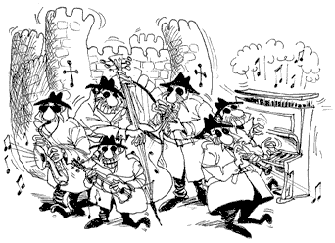
\includegraphics[scale=0.5]{Figures/BouncyCastle}
   \decoRule
   \caption[Legion of Bouncy Castle]{The Legion of Bouncy Castle, creadores de Bouncy Castle}
   \label{fig:BouncyCastle}
 \end{figure}

 %----------------------------------------------------------------------------------------

 \section{Padding}

 \keyword{Padding} es el nombre que recibe la técnica que permite en criptografía por bloques expandir el último bloque del mensaje hasta lograr el tamaño requerido.

 Existen múltiples técnicas de padding. Bruce Schenier, en su libro \emph{Cryptography Engineering}, menciona dos:
 \begin{itemize}
 \item Agregar al final del mensaje un byte con el valor 128 y luego agregar tantos 0’s como haga falta para alcanzar el largo del \emph{bloque de largo fijo}.
 \item Determinar el número de bytes que se requieren de padding. Supongamos que este número es \keyword{n}. Completar el mensaje con \keyword{n} bytes de valor \keyword{n}.
 \end{itemize}

 Cualquier técnica es válida mientras permita completar el mensaje hasta el largo requerido y el receptor pueda obtener con exactitud el mensaje original. \emph{\parencite{Reference8}}

 %----------------------------------------------------------------------------------------

 \section{Criptografía de clave pública}

 La \keyword{criptografía de clave pública}, también llamada criptografía asimétrica, es el método criptográfico que usa un par de claves para la firma y el cifrado de mensajes.
 Una clave es \emph{pública} y se puede entregar a cualquier persona, la otra clave es \emph{privada} y el propietario debe guardarla de modo que nadie tenga acceso a ella.

 Si el remitente usa la clave pública del destinatario para cifrar el mensaje, una vez cifrado, sólo la clave privada del destinatario podrá descifrar este mensaje, ya que es el único que la conoce.
 Por tanto se logra la \emph{confidencialidad} del envío del mensaje, nadie salvo el destinatario puede descifrarlo.

 Si el propietario del par de claves usa su clave privada para cifrar el mensaje, cualquiera puede descifrarlo utilizando su clave pública.
 En este caso se consigue por tanto la \emph{identificación} y \emph{autentificación} del remitente, ya que se sabe que sólo pudo haber sido él quien empleó su clave privada (salvo que alguien se la hubiese podido robar).
 Esta idea es el fundamento de la firma electrónica\footnote{Existen multitud de algoritmos de firma, para este proyecto se ha optado por usar RSASSA-PSS.}. \emph{\parencite{Reference5}}

 \begin{figure}[ht]
   \centering
   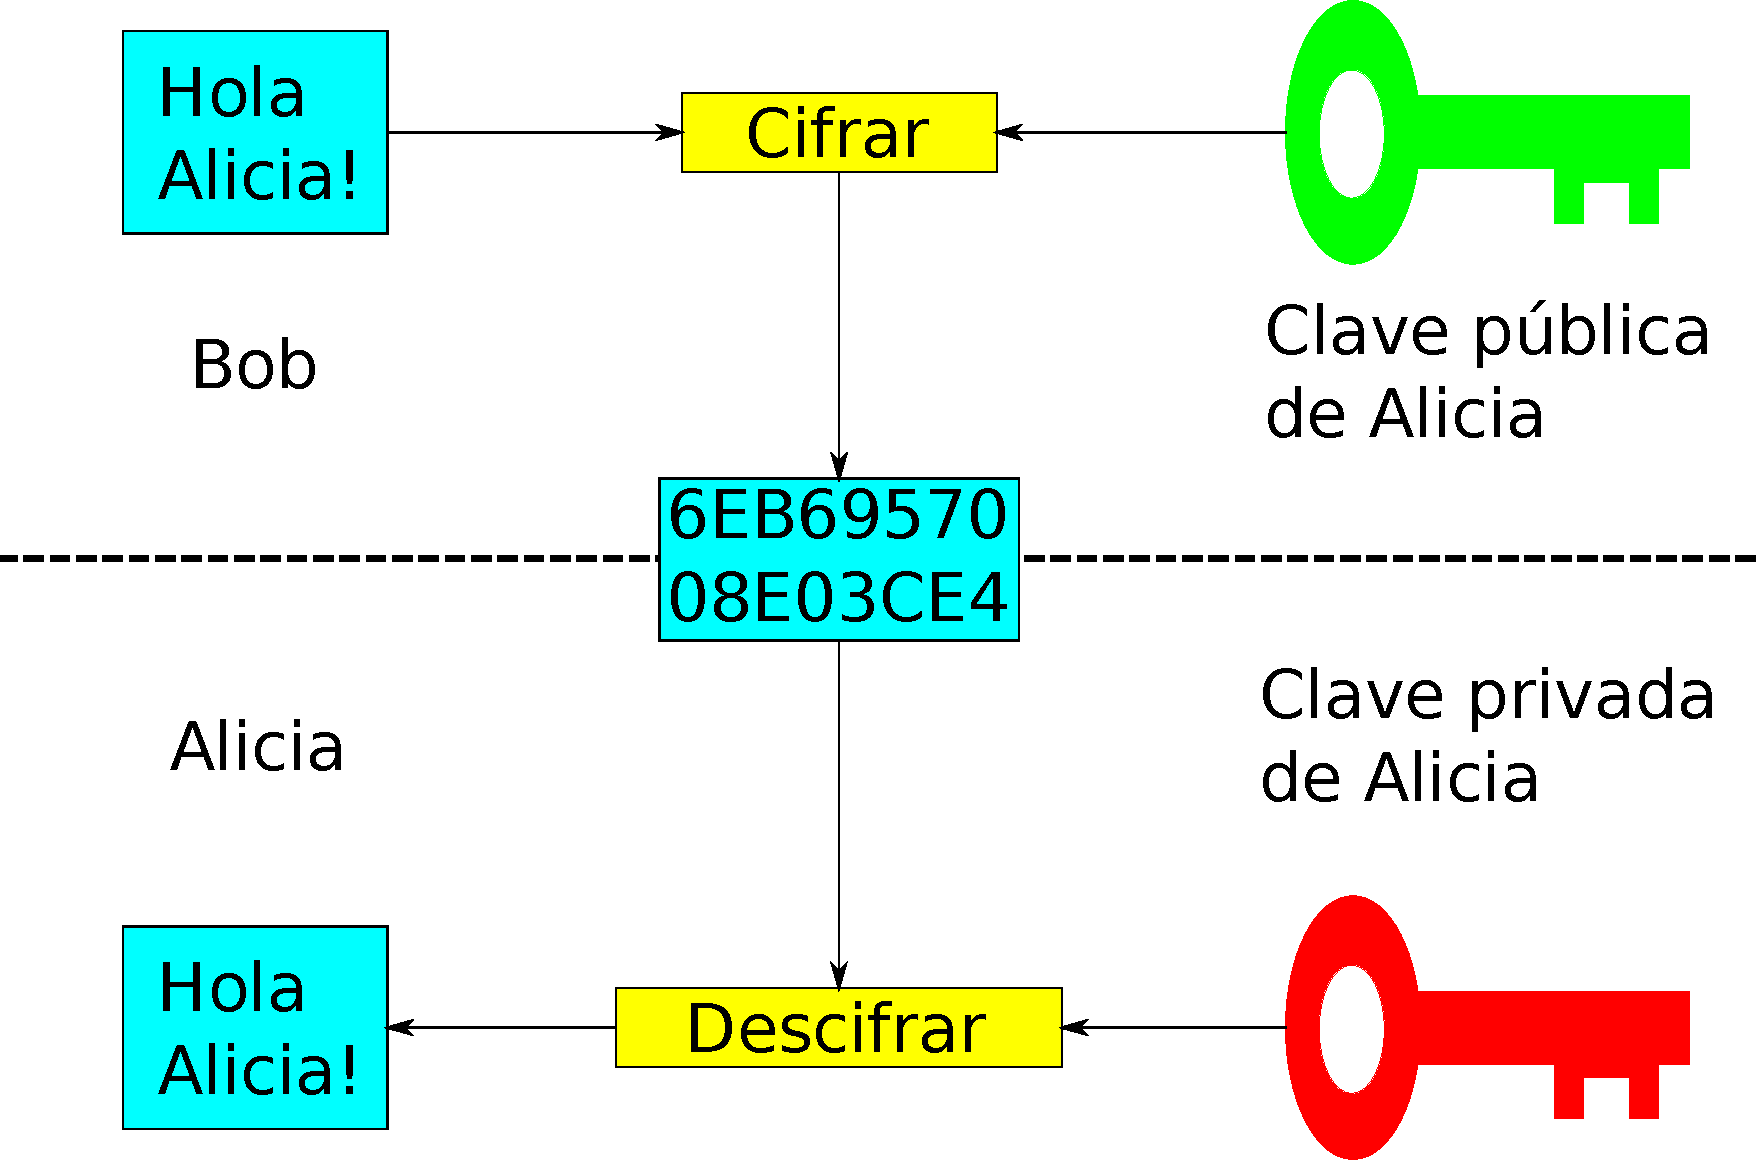
\includegraphics[scale=0.5]{Figures/PublicKeyEncryption}
   \decoRule
   \caption[Cifrado de clave pública (Esquema)]{Esquema general del cifrado de clave pública}
   \label{fig:PublicKeyEncryption}
 \end{figure}

 %----------------------------------------------------------------------------------------

 \section{RSA}

 \keyword{RSA} (\keyword{Rivest–Shamir–Adleman})\footnote{El acrónimo RSA está compuesto por las letras iniciales de los apellidos de Ron Rivest, Adi Shamir y Leonard Adleman, quienes primero describieron públicamente el algoritmo en 1978.} es uno de los primeros sistemas de criptografía de clave pública y es ampliamente utilizado para la transmisión segura de datos.
 En RSA, la asimetría que existe entre las claves pública y privada se basa en la dificultad práctica de la factorización del producto de dos grandes números primos (\emph{factoring problem}). \emph{\parencite{Reference9}}

 \subsection{Clave pública RSA}

 Una \keyword{clave pública RSA} consta de dos componentes:
 \begin{itemize}
 \item \keyword{n} -- el módulo RSA, un entero positivo.
 \item \keyword{e} -- el exponente público RSA, un entero positivo.
 \end{itemize}

 En una \keyword{clave pública RSA} válida, \keyword{n} es un producto de \keyword{u} números primos impares distintos
 \[ r_i, i = 1, 2, ..., u \]
 , donde \keyword{u} >= 2, y \keyword{e} es un entero entre 3 y \keyword{n} - 1, satisfaciendo
 \[ MCD(e, \lambda(n)) = 1 \]
 , donde
 \[ \lambda(n)\footnote{Función de Carmichael.} = mcm(r_1 - 1, ..., r_u - 1) \]
 Por convención, los dos primeros números primos se denotan como \emph{p} y \emph{q}, respectivamente.\footnote{La ventaja de usar más de dos números primos es que tendríamos un menor coste computacional para el desencriptador.} \emph{\parencite{Reference10}}

 \subsection{Clave privada RSA}

 Una \keyword{clave privada RSA} consta de dos componentes:\footnote{Existe otra representación de una clave privada que consta de un quinteto de factores, pero para este proyecto se ha usado la representación que se detalla.}
 \begin{itemize}
 \item \keyword{n} -- el módulo RSA, un entero positivo.
 \item \keyword{d} -- el exponente privado RSA, un entero positivo.
 \end{itemize}

 En una \keyword{clave privada RSA} válida, el módulo \keyword{n} es el mismo que el correspondiente a la \keyword{clave pública}.
 El exponente privado \keyword{d} es un entero positivo menor que \keyword{n} que satisface
 \[ e * d = 1 \Mod{\lambda(n)} \]
 , donde \keyword{e} es el correspondiente exponente público RSA. \emph{\parencite{Reference11}}

 \subsection{Evaluación de la función RSA}

 Este es el proceso de transformar un mensaje de texto plano en texto cifrado, o viceversa.
 La \keyword{función RSA}, para el mensaje \emph{m} y la clave \emph{k} se evalúa de la siguiente manera:
 \[ F(m, k) = m^k \Mod{n} \]

 Hay obviamente dos casos:
 \begin{itemize}
 \item Cifrar con la \emph{clave pública} y luego descifrar con la \emph{clave privada}.
 \[ F(m, e) = m^e \Mod{n} = c \]
 \[ F(c, d) = c^d \Mod{n} = m \]
 , donde \emph{m} es el mensaje\footnote{El mensaje se representa como un número entero mediante una transformación, que convierte el bytecode(Hexadecimal) a decimal.}, \emph{e} es el exponente público, \emph{d} es el exponente privado y \emph{c} es el mensaje cifrado.
 \item Cifrar con la \emph{clave privada} y luego descifrar con la \emph{clave pública}.
 \end{itemize}

 Ambos casos son un espejo del otro, y las funciones de encriptación y desencriptación son equivalentes. \emph{\parencite{Reference12}}

 %----------------------------------------------------------------------------------------

 \section{RSASSA-PSS}

 %----------------------------------------------------------------------------------------

 \section{Criptografía de clave simétrica}

 %----------------------------------------------------------------------------------------

 \section{Cifrado de bloques}

 %----------------------------------------------------------------------------------------

 \section{CBC}

 %----------------------------------------------------------------------------------------

 \section{AES}

 %----------------------------------------------------------------------------------------

 \section{HTTP}
